%!TEX root = ../cluster_semi.tex
\section{Background}
\label{sec:background-and-challenges}

\subsection{Anomaly Detection for KPI Streams}
\label{subsec:problem}
A KPI stream of an Internet-based service is a time series with the format of (timestamp, value). It is essentially monitoring data collected from Simple Network Management Protocol (SNMP), syslogs, web access logs or other data sources~\cite{meng2018device,zhang2018prefix,zhang2017syslog}. 
It can be denoted as $x_{t-m+1}, \dots, x_t$, where $x_i$ is a monitoring value at time $i, i\in[t-m+1, t]$, $t$ is the present time, and $m$ is the length of the KPI stream.

Anomalous data points of a KPI stream usually have different data characteristics from those of normal data points.
For example, a spike, a level shift or a dip in a KPI stream likely indicates an anomaly.
Figure~\ref{fig:anomaly} shows three examples of anomalies in KPI streams.
Anomaly detection for the KPI stream $x_{t-m+1}, \dots, x_t$ is to determine whether $x_t$ is an anomalous data point (let $y_t=1$ denote an anomalous data point and $y_t=0$ denote a normal one). 

\begin{figure}
\setlength{\abovecaptionskip}{-0.1cm}
      \begin{minipage}[h]{1.0\linewidth}
      \centering
      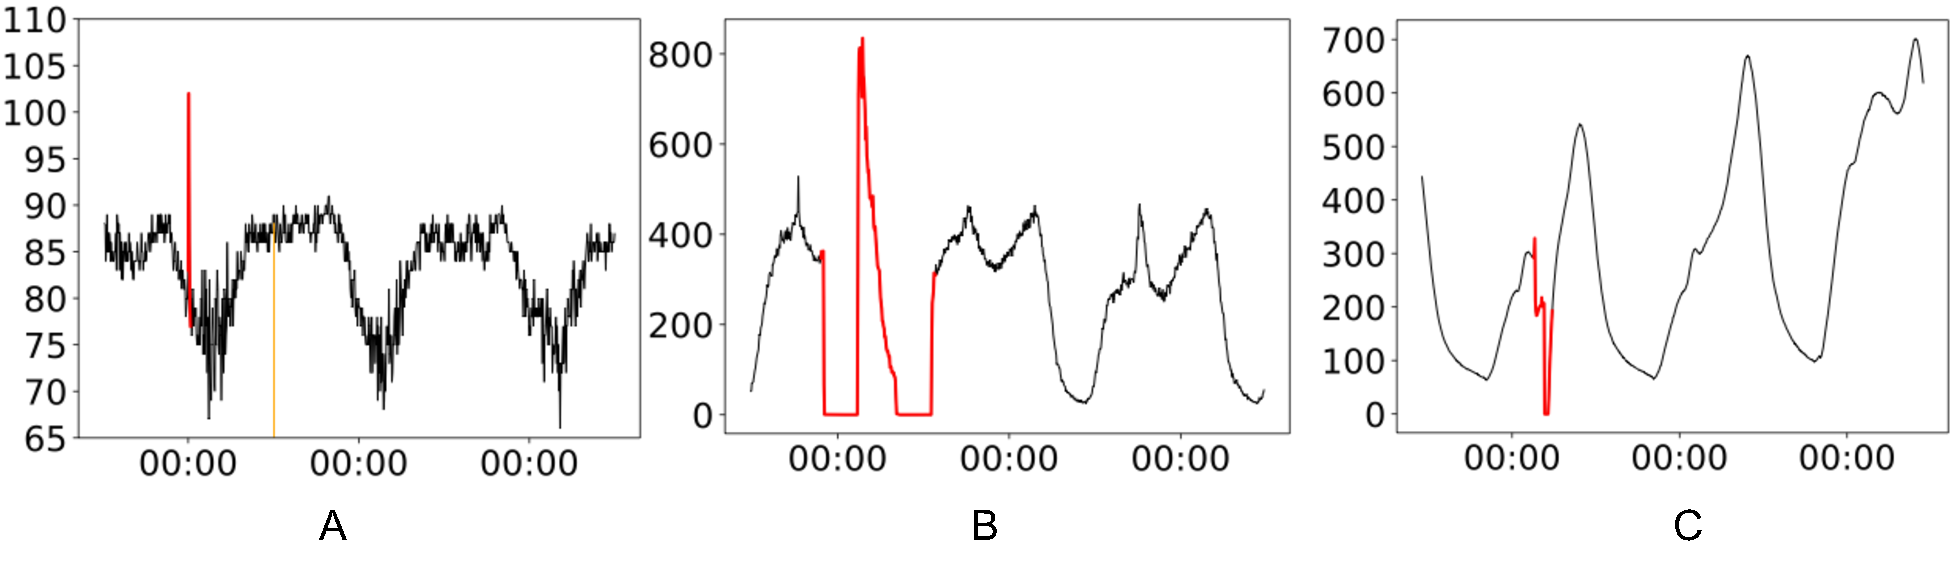
\includegraphics[width=1\textwidth]{fig/anomaly.pdf}\\
      \end{minipage}
      %\vspace{-5 mm}
      \caption{Examples of anomalies in KPI streams. 
      The red parts in the KPI stream denote anomalous points, and the orange part denotes missing points (filled with zeros).
      % anomalous data points are marked as red, and missing points (filled with zeros) are marked as orange.
      }
      \label{fig:anomaly}
      \vspace{-6 mm}
\end{figure}


 Most anomaly detection algorithms, including traditional statistical algorithms, supervised learning based methods and unsupervised learning based methods, compute an anomaly score for a data point to denote how likely this data point is anomalous.
 Operators then set a threshold to determine whether each data point is anomalous or not. 
 That is, only if the anomaly score at time $t$ exceeds this threshold, $x_t$ will be regarded as an anomalous data point.
% Examples of KPI streams are shown in Fig.~\ref{fig:anomaly}.

From the above definition, we can see that anomaly detection for a KPI stream is essentially a two-class classification problem -- classifying a data point into an anomalous data point or a normal one. 
Consequently, we can use the intuitive classification metrics of two-class classification methods, including precision, recall, and F-score, to evaluate the performance of anomaly detection algorithms.
 % for example, recall, precision, Precision-Recall curve, F-score, and so on.

% \subsection{Application Scenario}
% \label{subsec:challenges}
\subsection{Anomaly Detection Methods for KPI Streams}
\label{sec:related}
Anomaly detection for KPI streams deals with the task of recognizing unexpected data points from normal behavior.
Over the years, diverse \emph{traditional statistical algorithms} have been applied for KPI anomaly detection, including SVD~\cite{Mahimkar:2011:RDM:2079296.2079309}, Wavelet~\cite{barford2002signal}, ARIMA~\cite{Zhang:2005:NA:1251086.1251116}, Time Series Decomposition~\cite{chen2013provider}, Holt-Winters~\cite{yan2012argus}, \emph{etc.}
Each of the above algorithms computes an anomaly score for each data point in a KPI stream on the basis of simple statistical assumptions. 
To achieve the best accuracy, operators have to manually select an anomaly detection algorithm and tune its parameters for \emph{each KPI stream}.
Since it is often the case that a large number of newly emerging KPI streams have to be carefully monitored~\cite{zhang2016funnel}, manual \textbf{algorithm selection and parameter tuning} for every newly emerging KPI stream becomes infeasible.

To address the problem posed by algorithm selection and parameter tuning, several \emph{supervised learning} based methods such as EGADS~\cite{egads} and Opprentice~\cite{liu2015opprentice} have been proposed.
For each KPI stream, these methods learn (traditional statistical) algorithm selection and parameter tuning from operators' manual labels of KPI anomalies.
Obviously, manual \textbf{anomaly labeling} for a large number of newly emerging KPI streams is not feasible either.

\emph{Unsupervised learning} has emerged as a promising field in KPI anomaly detection.
For example, isolation based methods~\cite{ding2013anomaly} and variational autoencoders (VAE)~\cite{xu2018unsupervised} are applied in detecting anomalies in (KPI) streams.
These methods are trained without manual labels, and thus they can be applied for large volume of KPI streams.
However, isolation based methods suffer from low accuracy~\cite{zhang2018anomaly} (see Section~\ref{subsec:overall-performance} for more details).
In addition, Donut~\cite{xu2018unsupervised}, which is based on VAE,
requires a long period (say six months) of training data for newly emerging KPI streams. 
During this period, the Internet-based services may suffer from false alarms (due to low precision) and/or missed alarms (because of low recall) and in turn impact user experience and revenue.

% For example, DONUT~\cite{xu2018unsupervised}, which is based on VAE, is trained based on six months worth of KPI stream data.

% These software upgrades and configuration changes likely generate \textbf{new KPI streams} or even new KPIs.
% If unsupervised learning based methods such as DONUT are applied to detect anomalies for these newly generated KPI streams, it will take a too long period (\emph{e.g.,} six months) to obtain an accurate anomaly detection model.
% During this period, the Internet-based service may suffer from false alarms (due to low precision) and/or missed alarms (because of low recall) and in turn impact on user experience and revenue.

As discussed above, existing anomaly detection algorithms for KPI streams suffer from manual algorithm selection and parameter tuning (traditional statistical algorithms), or manual anomaly labeling (supervised learning based methods), or low accuracy in real-world Internet-based service (unsupervised learning based methods like isolation forests~\cite{ding2013anomaly}), or long period of training time for newly generated KPI streams (unsupervised learning based methods like Donut~\cite{xu2018unsupervised}).

\emph{Semi-supervised learning}~\cite{chapelle2009semi} is halfway between supervised and unsupervised learning. It uses unlabeled data to modify either parameters or models obtained from labeled data alone to maximize the learning performance. ~\cite{rosenberg2005semi, ashfaq2017fuzziness, noto2012frac} use semi-supervised learning for anomaly detection in other domains, but are not designed for KPI streams (time series).

\subsection{Clustering of KPI Streams}
\label{subsec:background}
% Millions of KPI streams are continuously monitored in large Internet-based services, in order to timely mitigate the loss caused by incidents like server failures, network overload, malicious attacks, \emph{etc.}
Millions of KPI streams bring a huge challenge to KPI anomaly detection.
Luckily, many KPI streams are similar because of their implicit associations and similarities.
For example, Figure~\ref{fig:similar_curve} shows two KPI streams of response latency collected from two different applications, and these two KPI streams are quite similar in shape.
If we can identify similar KPI streams, and group the huge volume of KPI streams into a few clusters, we can reduce the overhead in anomaly detection.

% \begin{figure}
% 	\begin{subfigure}[t]{0.5\columnwidth}{}
% 		\centering
% 		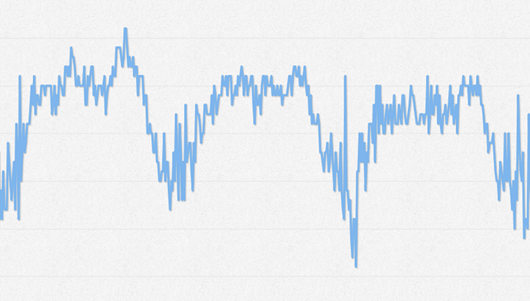
\includegraphics[width=.9\linewidth,height=28mm]{fig/curve1.png}
% 	\vspace{0.2em}{}
% 		\caption{Application 1}\label{fig:curve1}
% 	\end{subfigure}\hfill
% 	\begin{subfigure}[t]{0.5\columnwidth}
% 		\centering
% 		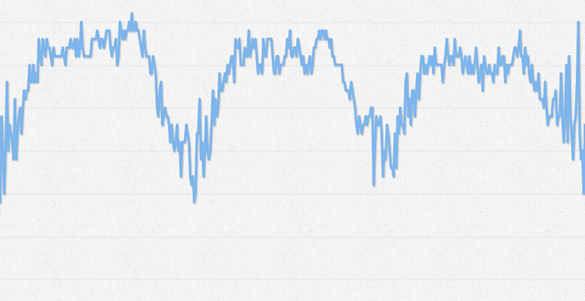
\includegraphics[width=.9\linewidth,height=28mm]{fig/curve2.png}
% 	\vspace{0.2em}
% 		\caption{Application 2}\label{fig:curve2}
% 	\end{subfigure}
% 	\caption{
% 		The latency streams of two different applications. 
% 	}
% 	\label{fig:similar_curve}
%     % \vspace{-1.2em}
% \end{figure}

\begin{figure}
\setlength{\abovecaptionskip}{-0.2cm}
      \begin{minipage}[h]{1.0\linewidth}
      \centering
      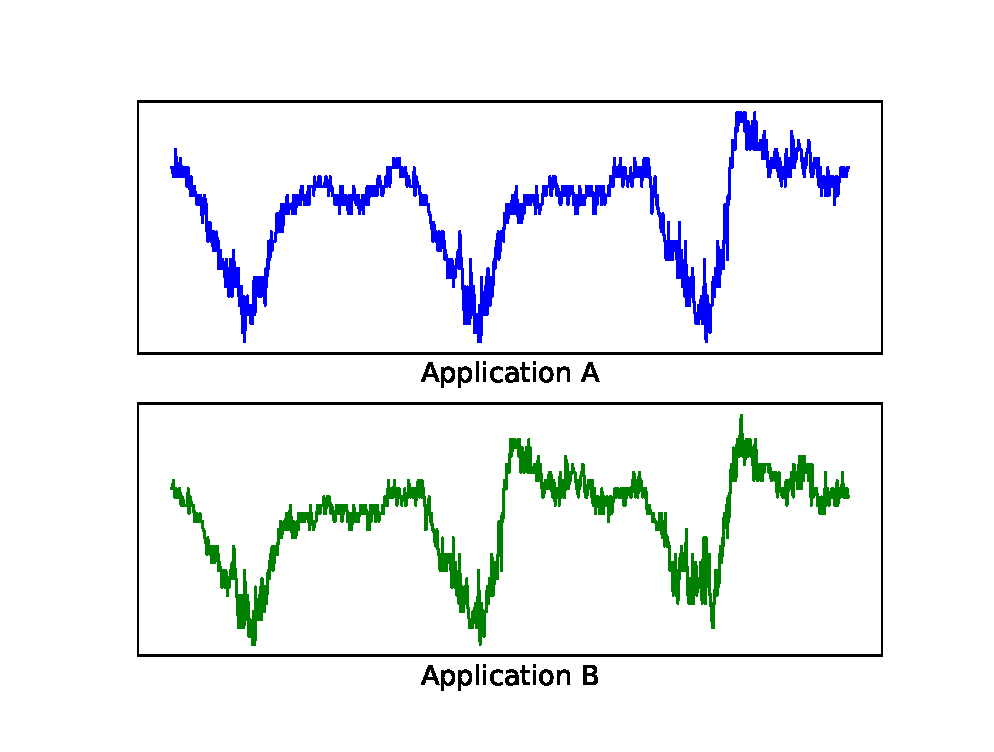
\includegraphics[width=0.9\textwidth]{fig/similar.eps}\\
      \end{minipage}
      %\vspace{-5 mm}
      \caption{The response latency streams of two different applications.
      }
      \label{fig:similar_curve}
     \vspace{-6 mm}
\end{figure}
% A famous company always operates hundreds of applications simultaneously and monitors millions of KPI streams. 
% Although the amount of KPI streams is huge, many KPI streams are homogeneous(\EG{}, the KPI streams of the same application from Mobile and PC). 
% Fig.~\ref{fig:similar_curve} show two latency streams collected from different applications. They have the similar shapes, which can be utilized in anomaly detection. 
% In this direction, we propose clustering and semi-supervised learning based methods.

Time series clustering is a popular field which has caught lots of attention in the past 20 years. 
\cite{liao2005clustering} summarized a large number of methods on this topic, most of which are designed for smooth and idealized data.
However, the large number of spikes, dips and level shifts in KPI streams can significantly 
change the shape of KPI streams. 
Therefore, the above methods do not perform good for KPI streams.
% In addition, some of these techniques have high computation complexity~\cite{sakoe1978dynamic}. 
% Another famous method is YADING~\cite{ding2015yading}, but it will take most KPI streams as outliers which mean they are different from each other. 

In this work, we adopt \ROCKA~\cite{lirobust}, a rapid clustering algorithm for KPI streams based on their shapes. 
It applies moving average to extract baselines which successfully reduce the biases of noises and anomalies. 
In addition, it uses shape-based distance
% (SBD)~\cite{paparrizos2015k} 
as the distance measure, and reduces its algorithm complexity to $O(m\log(m))$ using Fast Fourier Transform. 
Finally, it uses DBSCAN
% ~\cite{ester1996density} 
to cluster KPI streams and chooses the centroid for every cluster. 
Extensive experiments in~\cite{lirobust} have demonstrated ROCKA's superior performance in clustering KPI streams for large Internet-based services. 
% We simply apply this clustering algorithm and do not improve it.
Please note that applying ROCKA to cluster KPI streams is not our contribution.

% Besides the ROCKA clustering algorithm, \cite{lirobust} also trains a Donut~\cite{xu2018unsupervised} model on a given cluster centroid and uses this model to detect anomalies on the other KPI streams belonging to the same cluster, whose average F-scores degrade by 0.01 to 0.22 compared to the Donut models trained for each KPI stream. However, Donut typically requires large amounts of training data which is infeasible for the large number of newly emerging KPI streams in our scenario.


% Semi-supervised learning~\cite{zhou2014semi} is halfway between supervised and unsupervised learning. In reality, labeled data for a learning problem often requires a huge cost, so semi-supervised learning can be of great practical value. These methods use unlabelled data to modify either parameters or models obtained from labeled data alone to maximize the learning performance of the models. The basic questions of semi-supervised learning are whether the labelled data is useful and how to utilize unlabelled data effectively. ~\cite{sillito2008semi, ashfaq2017fuzziness, noto2012frac} use semi-supervised learning for anomaly detection, but are not designed for KPI streams (time series).

% In our research scenario, KPI streams can be grouped into a few clusters based on their shapes. The data points on similar shape KPI streams always have similar data distribution, so we can train semi-supervised learning model on KPI streams belonging to the same cluster. The clustering is the premise while the semi-supervised learning is the core of \name{}.

